% As outras 14 instituições aparecem uma vez cada; o gráfico destaca as recorrências.
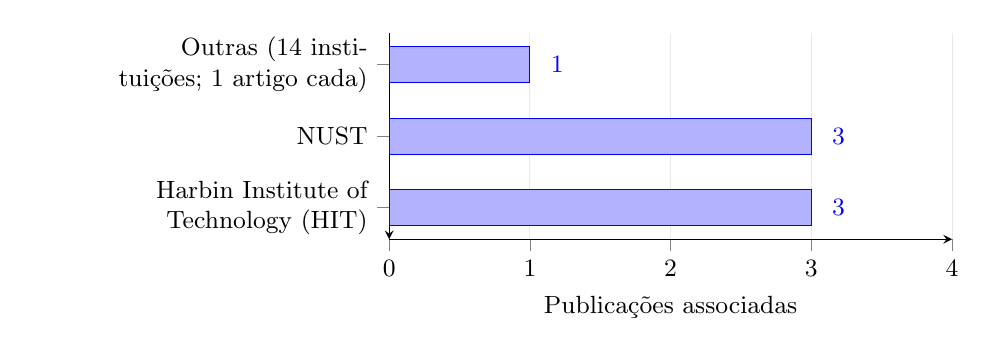
\begin{tikzpicture}
\begin{axis}[
  xbar, width=0.72\textwidth, height=4.2cm,
  xmin=0, xmax=4, xlabel={Publicações associadas},
  ytick={1,2,3},
  yticklabels={Outras (14 instituições; 1 artigo cada),NUST,Harbin Institute of Technology (HIT)},
  y dir=reverse, xtick={0,1,2,3,4},
  axis lines=left, tick align=outside,
  xmajorgrids=true, grid style={gray!18},
  tick label style={font=\small}, label style={font=\small},
  yticklabel style={font=\small, text width=4.2cm, align=right},
  nodes near coords, nodes near coords style={font=\small\bfseries, xshift=4pt},
  bar width=13pt, enlarge y limits=0.22,
  every axis plot/.append style={fill=teal!65!blue, draw=teal!65!blue!80!black}
]
\addplot coordinates {(1,1) (3,2) (3,3)};
\end{axis}
\end{tikzpicture}
